% LINGI2255 - Software Development Project
% Manual
\documentclass{article}
\usepackage[utf8]{inputenc}
\usepackage[UKenglish]{babel}
\usepackage{graphicx}

\title{Manual}


\usepackage{caption}% http://ctan.org/pkg/caption
\captionsetup[figure]{labelformat=empty}%

\title{Care4Care: User Manual}

\author{Group 8 \\ 
\\
Baptiste Lacasse \\
Thibault Gerondal \\
Michaël Heraly \\
Denis Genon \\
Victor Velghe \\
Jeremy Vanhee \\
Arnold Moyaux \\
Aloïs Paulus}


\date{\today}

\begin{document}

\maketitle

\tableofcontents


\section{Introduction}
Welcome to Care4Care! In this document you will find how to use our application and the description of the database installed on http://care4demo.tycale.be.
 \section{User Manual}
 We will together discover the various features of the site Care4Care. In the various screenshots, the left mouse button is represented by a red dot. This help is available on the help page of the website.
\subsection{Sign in}
In order to use this website, you will need to make an account.
\begin{figure}[!ht]
   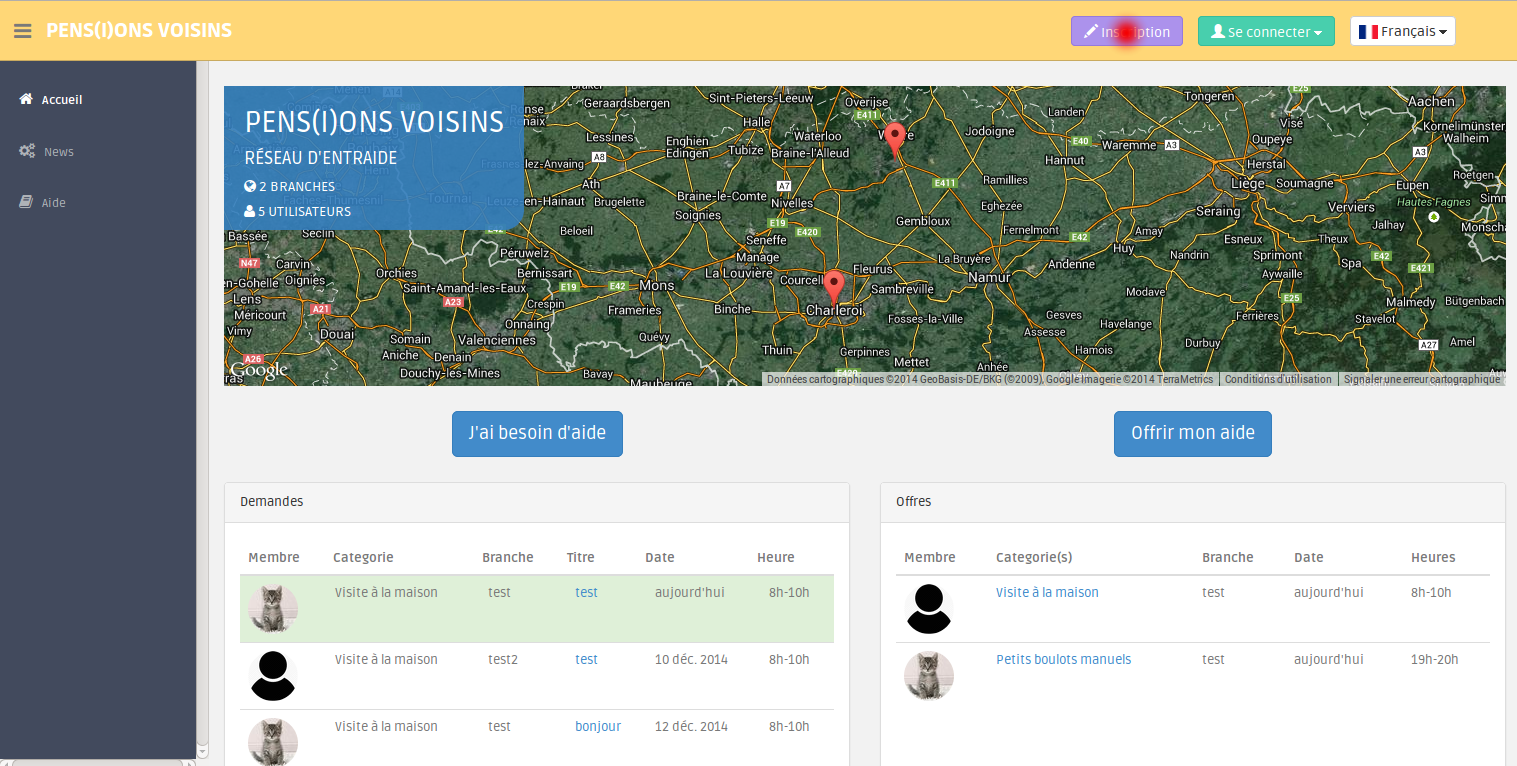
\includegraphics[width=\textwidth]{img/inscr1.png}
   \caption{Sign in: Step 1}
\end{figure}

\begin{figure}[!ht]
   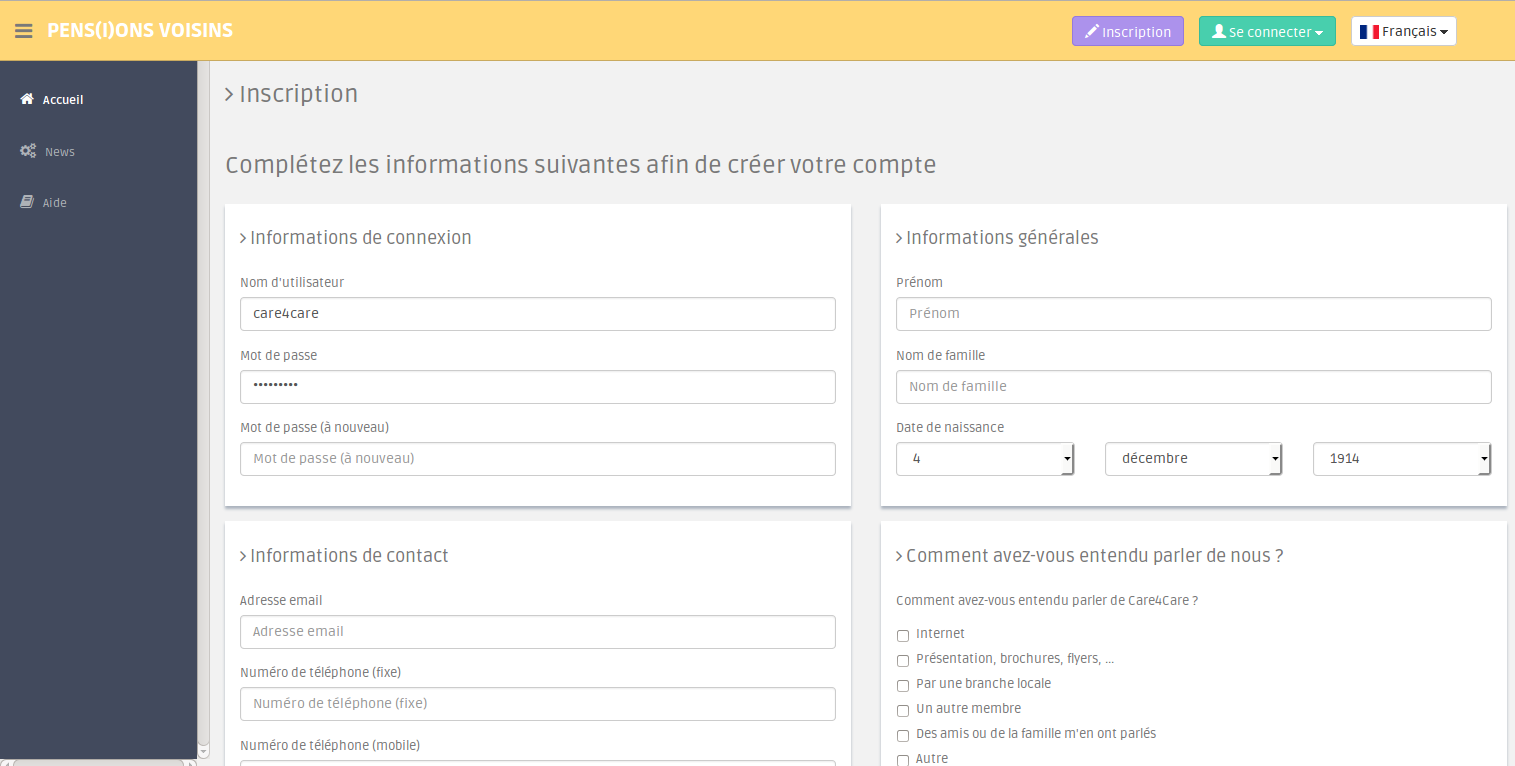
\includegraphics[width=\textwidth]{img/inscr2.png}
   \caption{Sign in: Step 2 - Fill in this form}
\end{figure}

\begin{figure}[!ht]
   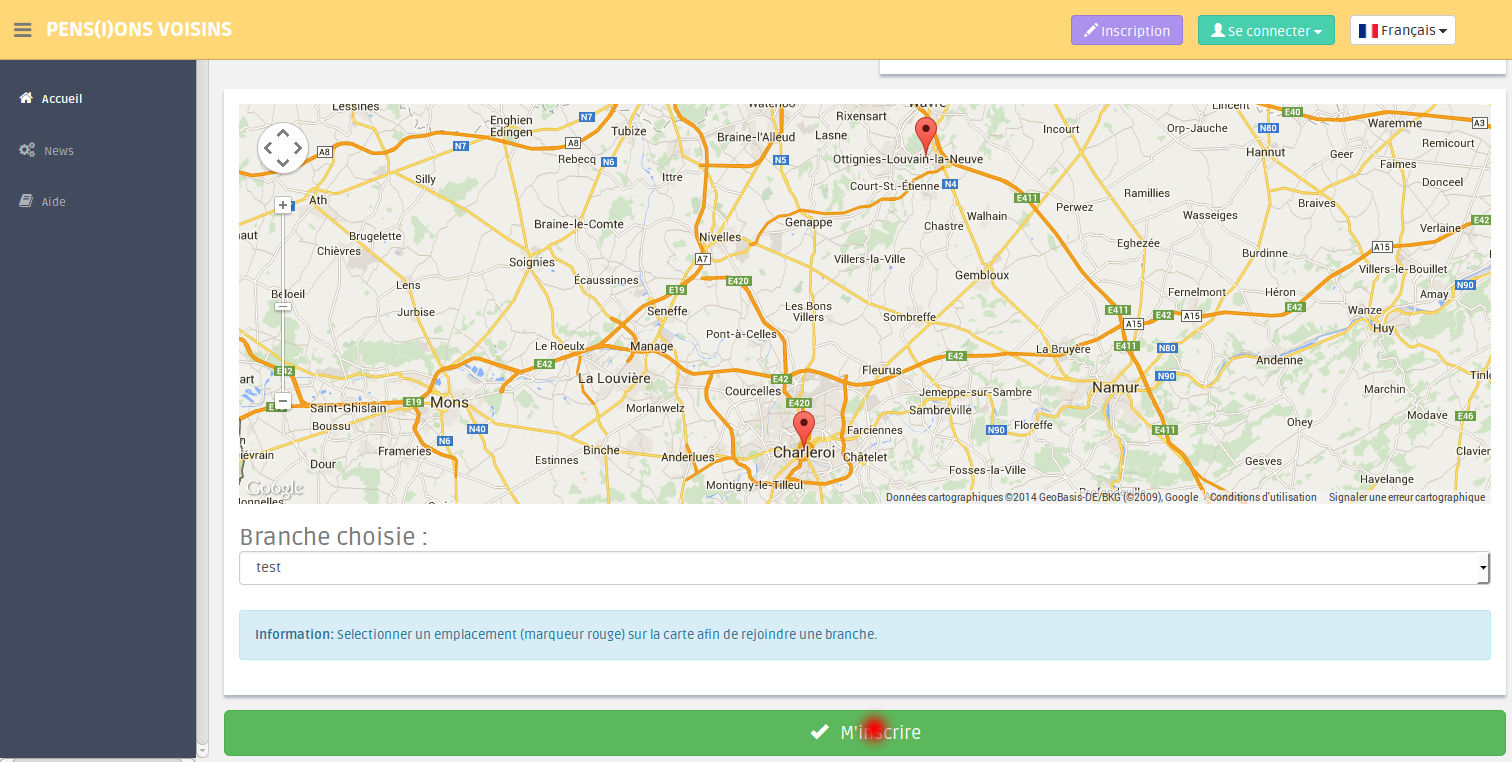
\includegraphics[width=\textwidth]{img/inscr3.png}
   \caption{Sign in: Step 3 - Send demand}
\end{figure}

\clearpage
\subsection{Display the menu}
The menu is used to navigate between each parts of the website.
\begin{figure}[!ht]
   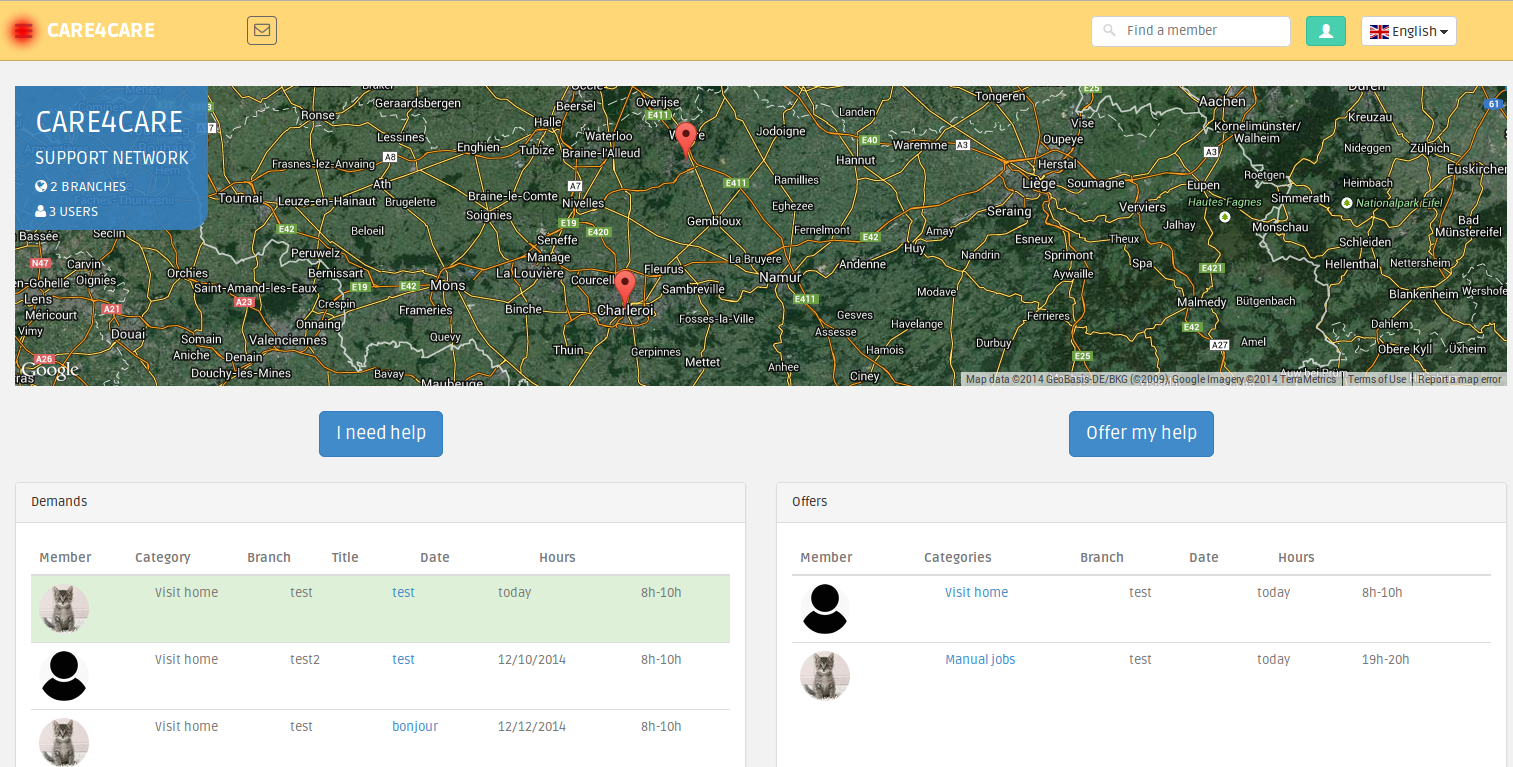
\includegraphics[width=\textwidth]{img/menu1.png}
   \caption{Menu: Step 1}
\end{figure}
\begin{figure}[!ht]
   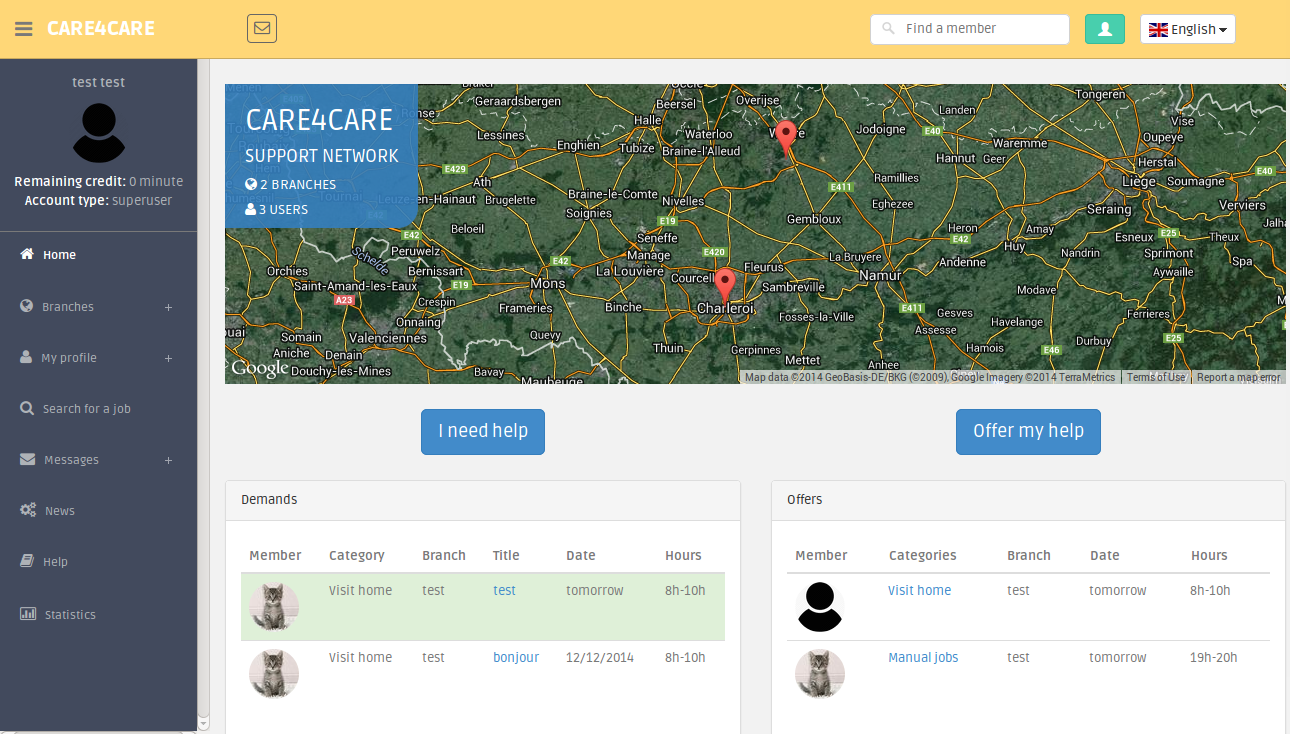
\includegraphics[width=\textwidth]{img/menu2.png}
   \caption{Menu: Result}
\end{figure}

\clearpage
\subsection{Sign out}
If you want to disconnect from the website, follow those steps.
\begin{figure}[!ht]
   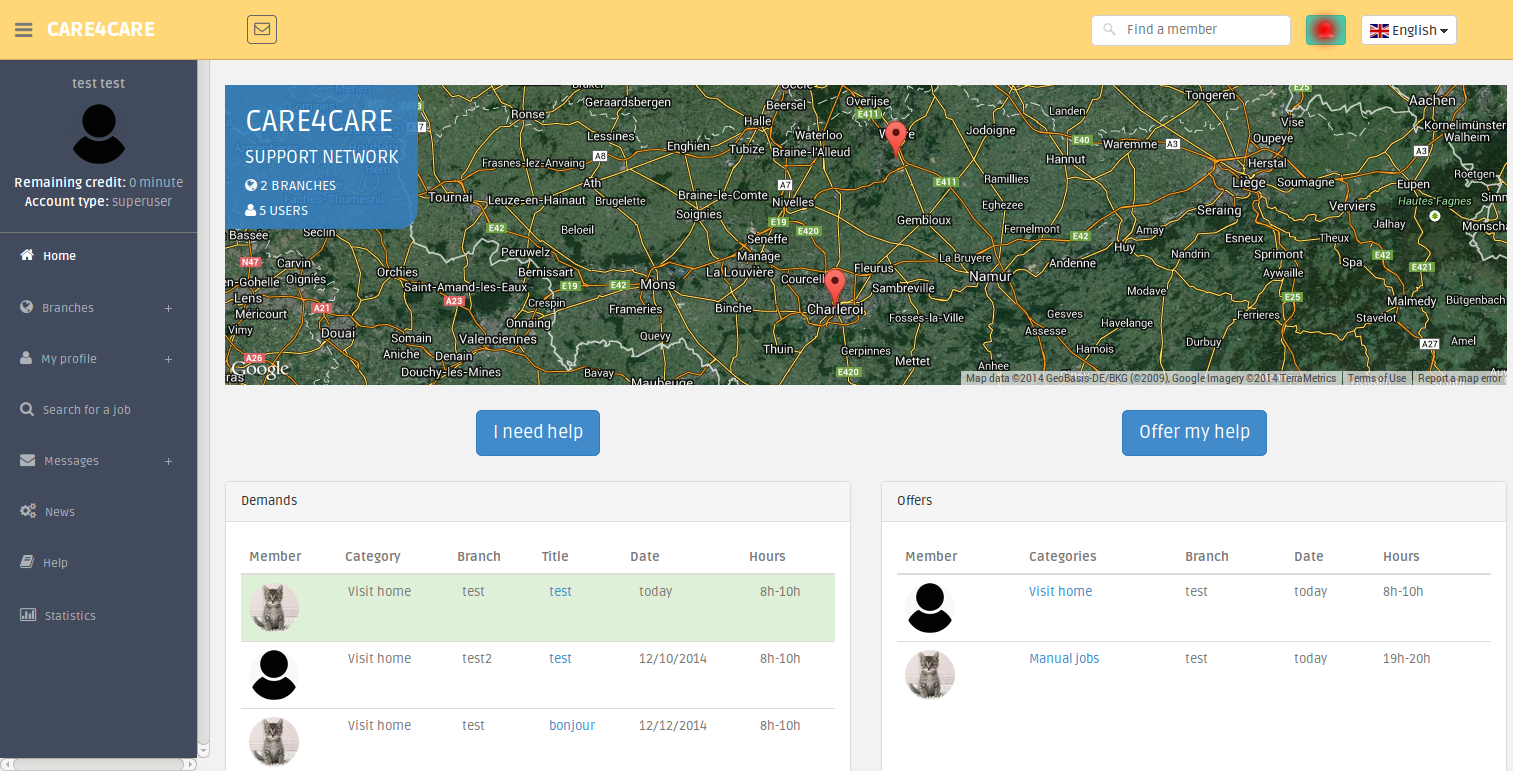
\includegraphics[width=\textwidth]{img/out1.png}
   \caption{Sign out: Step 1}
\end{figure}
\begin{figure}[!ht]
   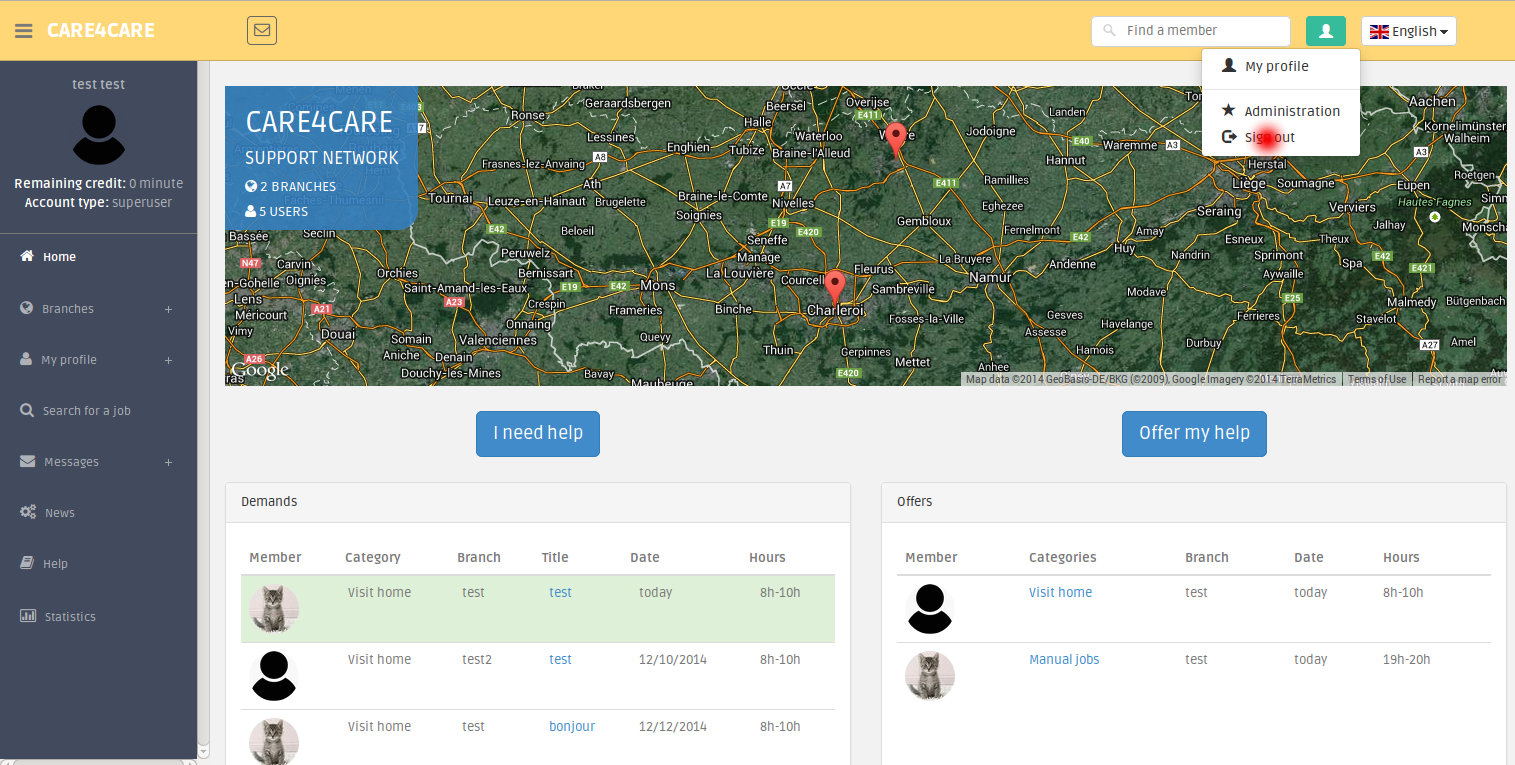
\includegraphics[width=\textwidth]{img/out2.png}
   \caption{Sign out: Step 2}
\end{figure}

\clearpage
\subsection{My profile}
Your profile contains all the informations about you needed for using Care4Care.
\subsubsection{Display my profile}
\begin{figure}[!ht]
   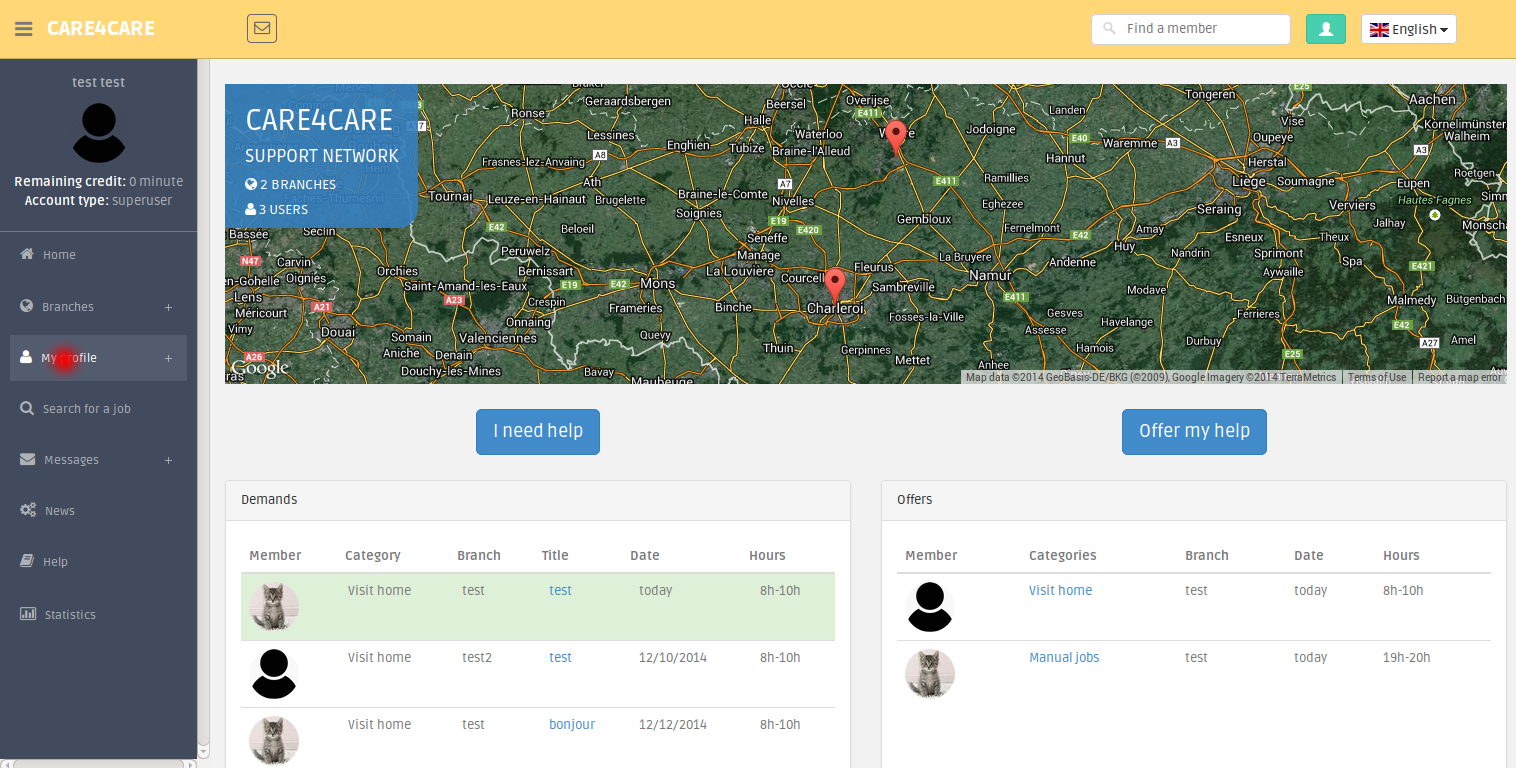
\includegraphics[width=\textwidth]{img/profil1.png}
   \caption{Display: Step 1}
\end{figure}
\begin{figure}[!ht]
   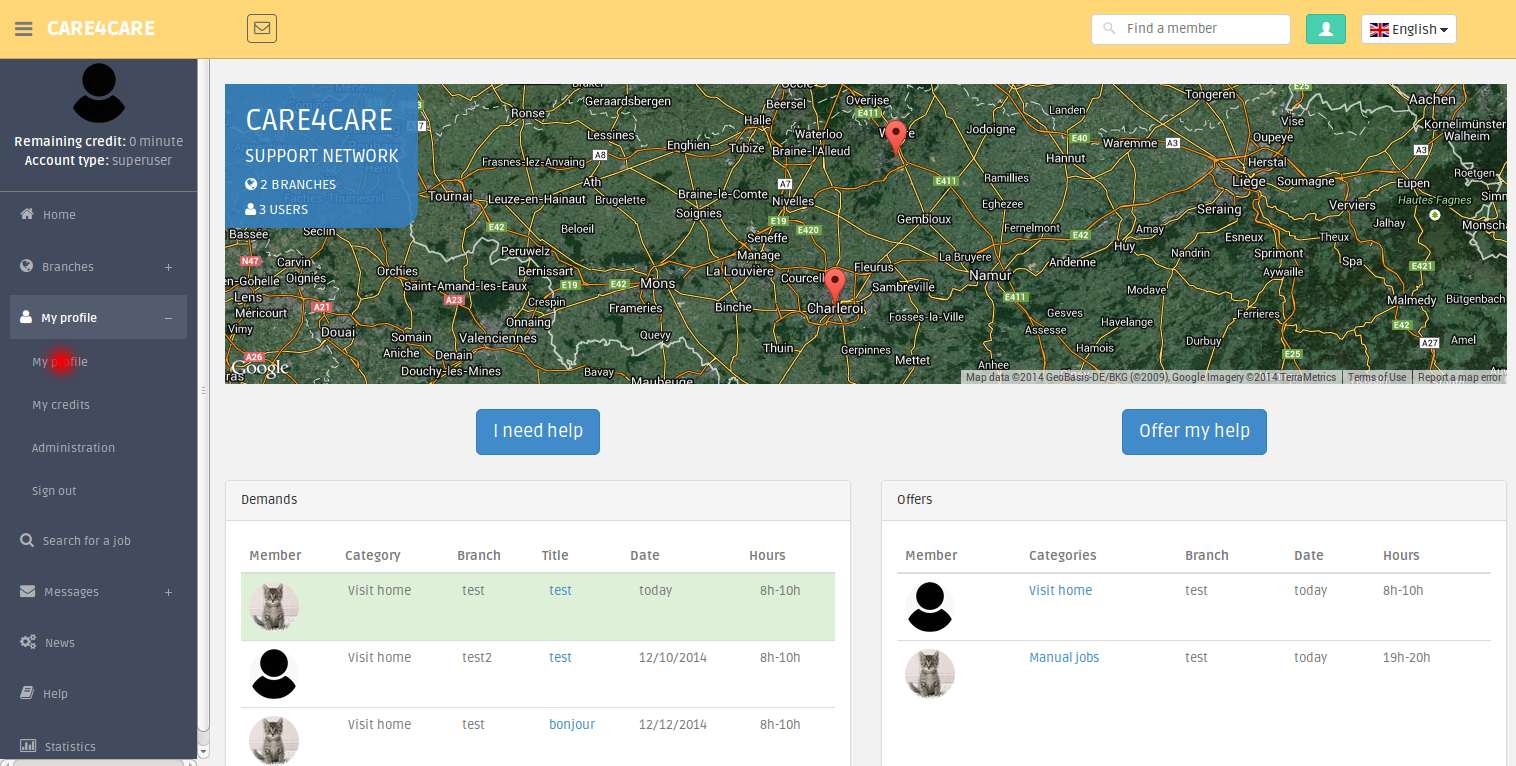
\includegraphics[width=\textwidth]{img/profil2.png}
   \caption{Display: Step 2}
\end{figure}
\begin{figure}[!ht]
   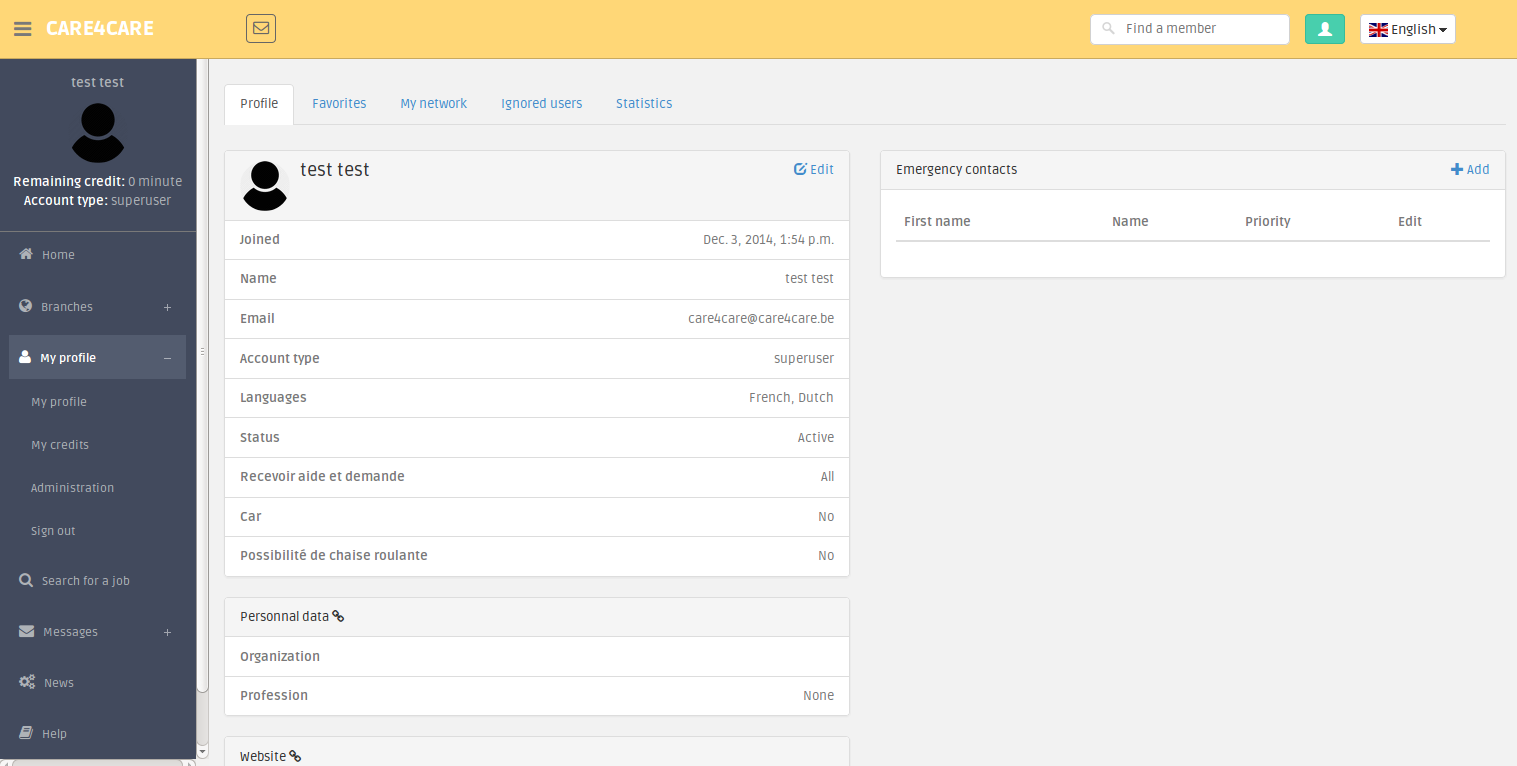
\includegraphics[width=\textwidth]{img/profil3.png}
   \caption{Display: Result}
\end{figure}

\clearpage
\subsubsection{Edit my profile}
Go to: \textbf{My profile}.
\begin{figure}[!ht]
   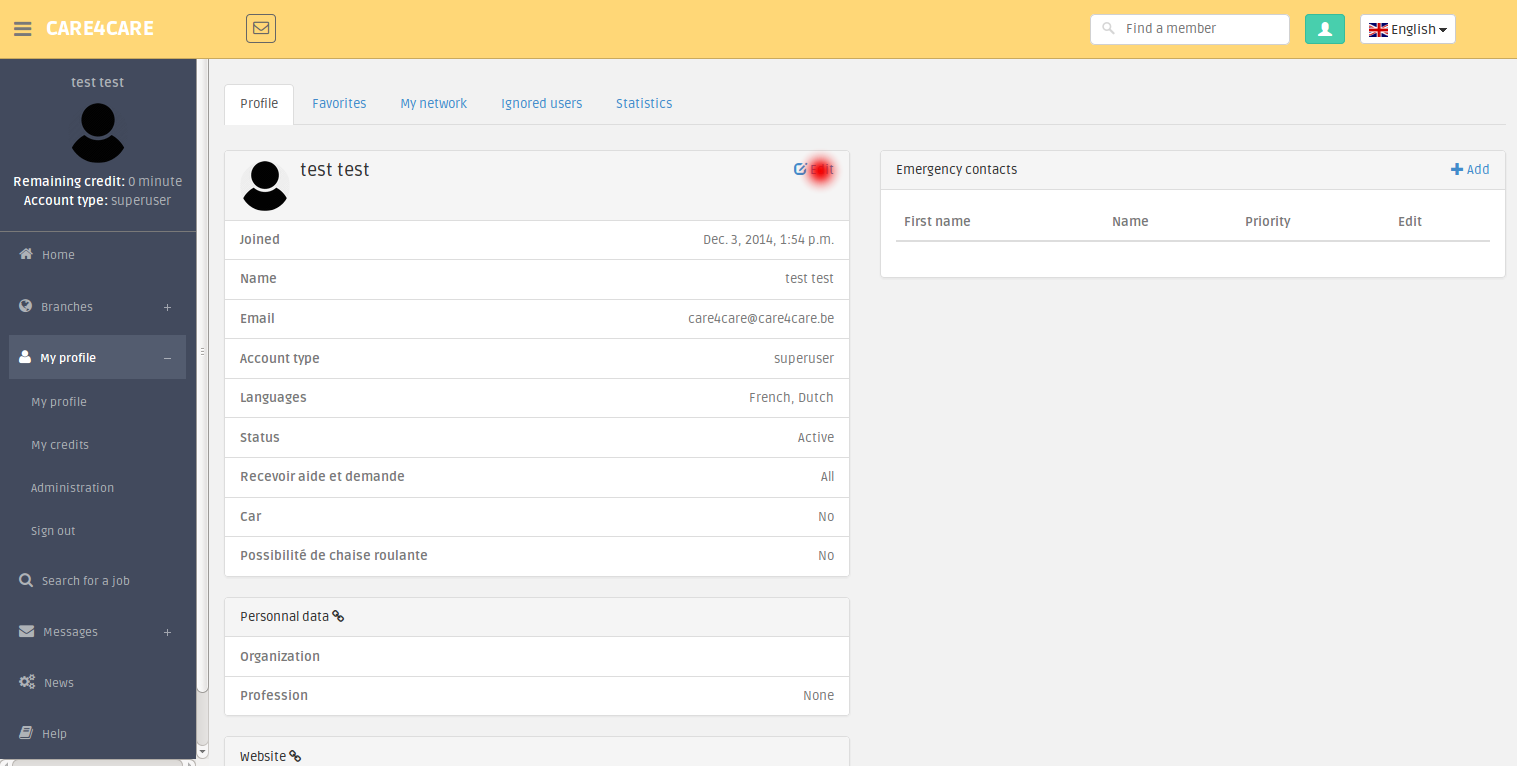
\includegraphics[width=\textwidth]{img/profil4.png}
   \caption{Edit: Step 1}
\end{figure}
\begin{figure}[!ht]
   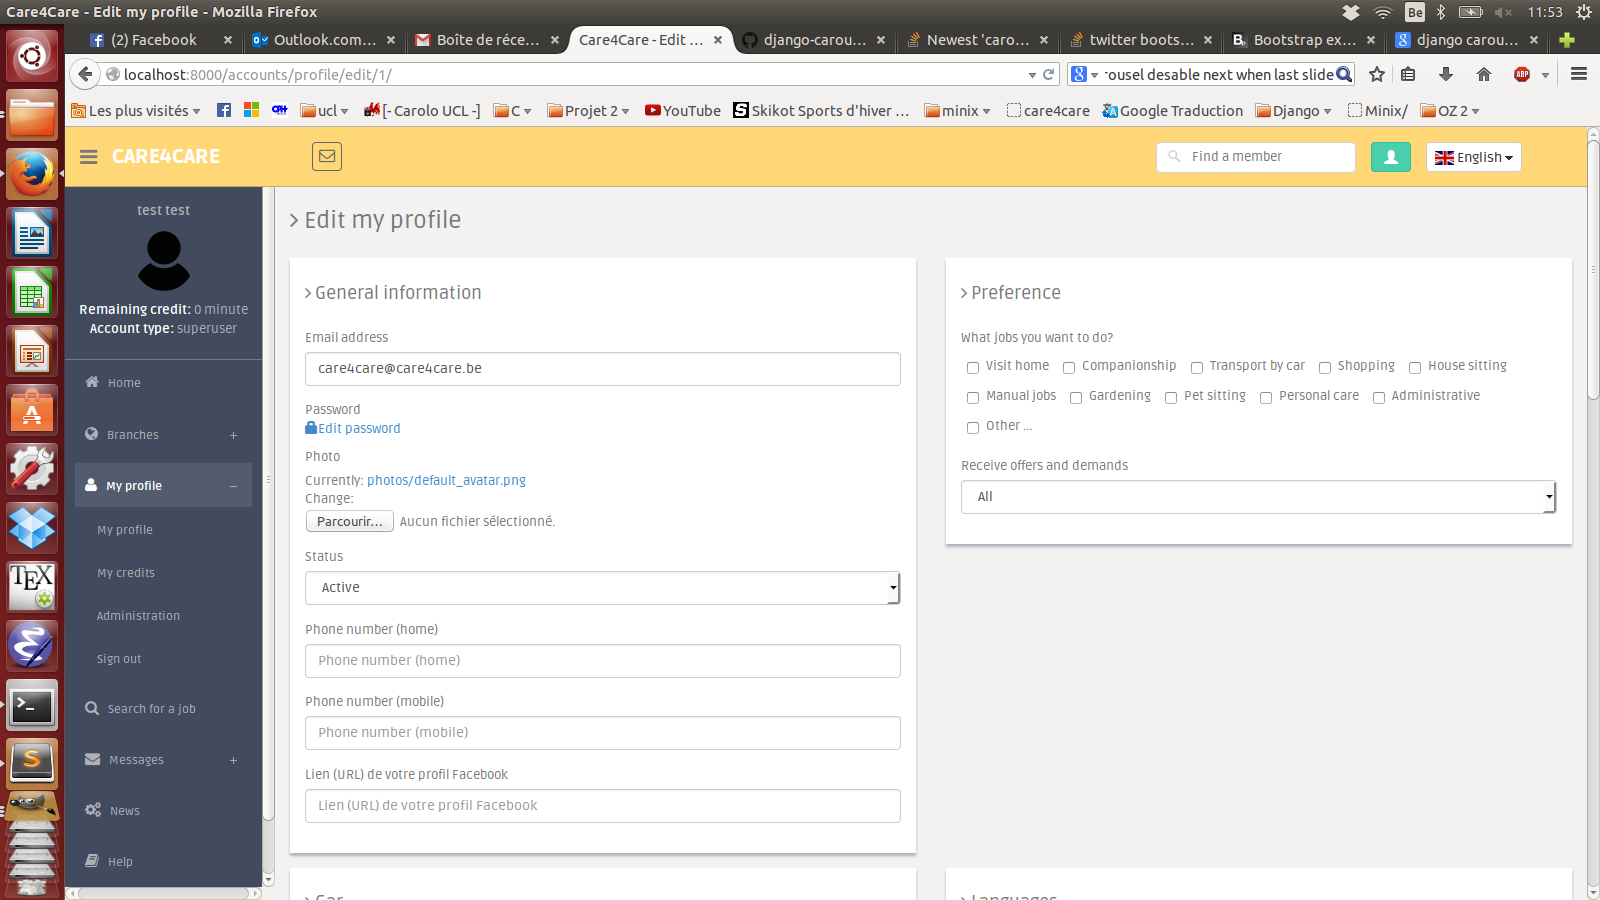
\includegraphics[width=\textwidth]{img/profil5.png}
   \caption{Edit: Step 2 - Fill in this form}
\end{figure}
\begin{figure}[!ht]
   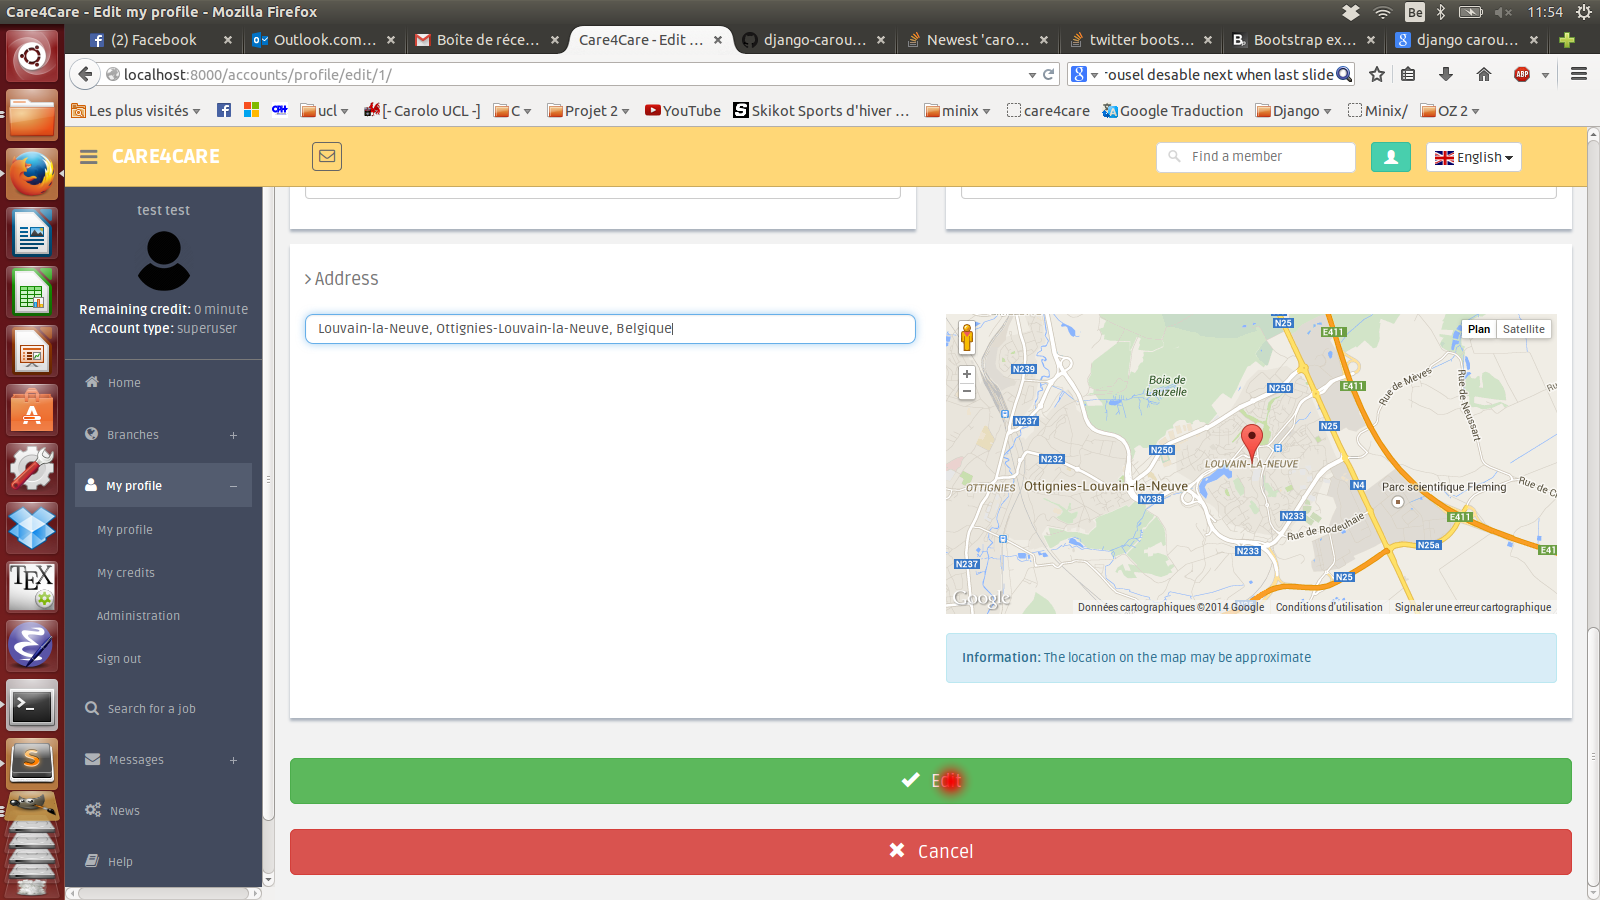
\includegraphics[width=\textwidth]{img/profil6.png}
   \caption{Edit: Step 3 - Send modifications}
\end{figure}

\clearpage
\subsection{Ask for help}

\begin{figure}[!ht]
   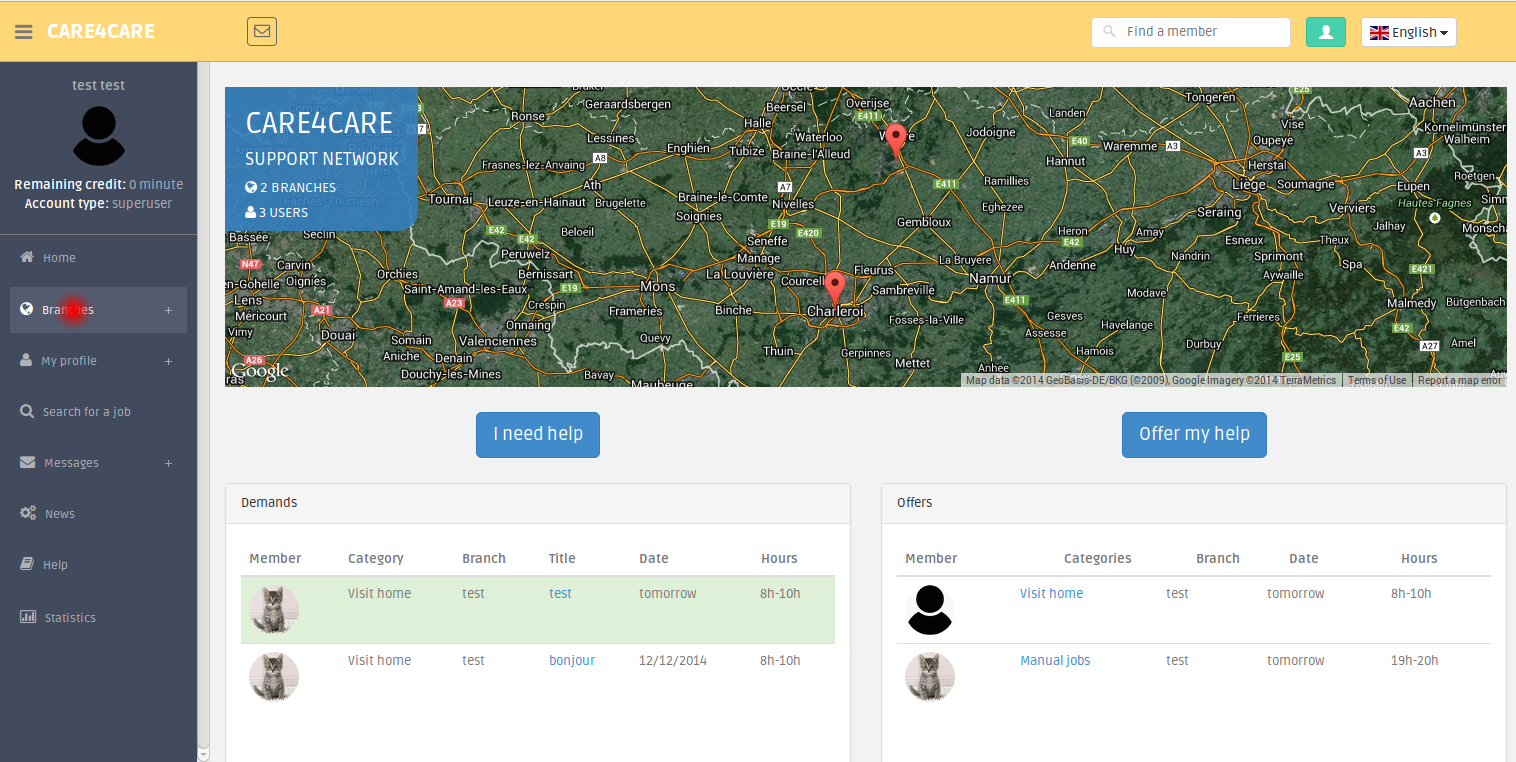
\includegraphics[width=\textwidth]{img/dem1.png}
   \caption{Ask: Step 1}
\end{figure}
\begin{figure}[!ht]
   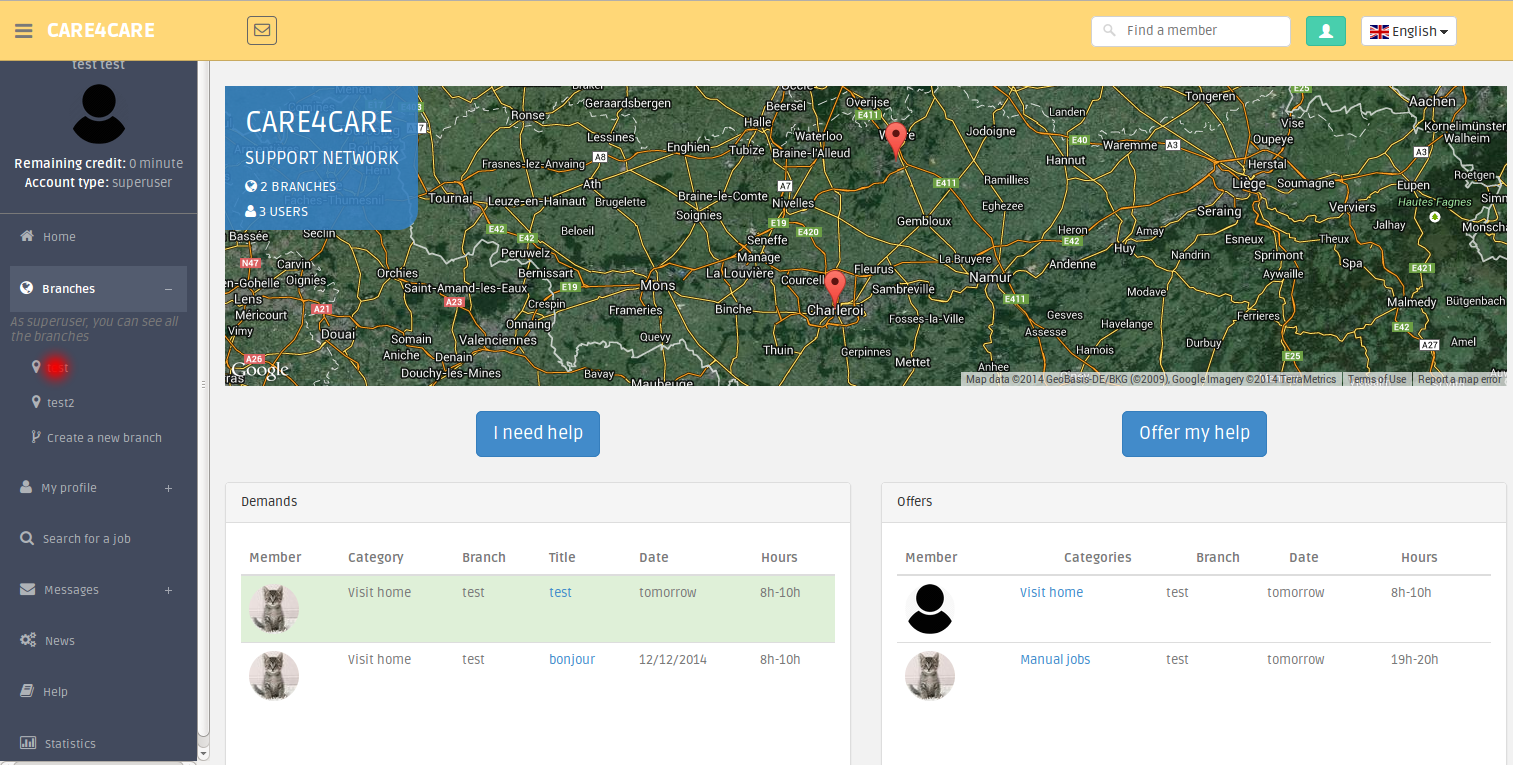
\includegraphics[width=\textwidth]{img/dem2.png}
   \caption{Ask: Step 2 - Choose a branch}
\end{figure}
\begin{figure}[!ht]
   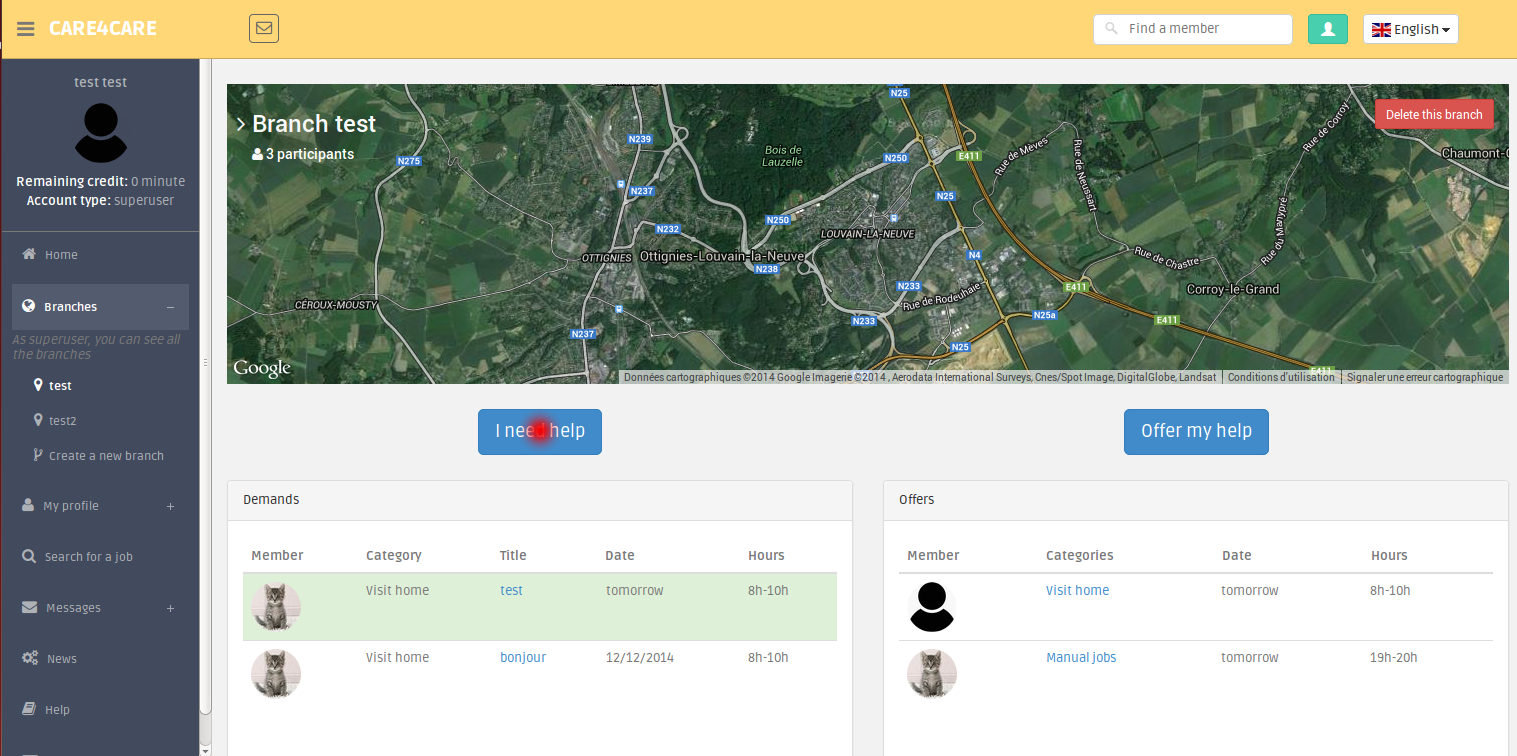
\includegraphics[width=\textwidth]{img/dem3.png}
   \caption{Ask: Step 3}
\end{figure}
\begin{figure}[!ht]
   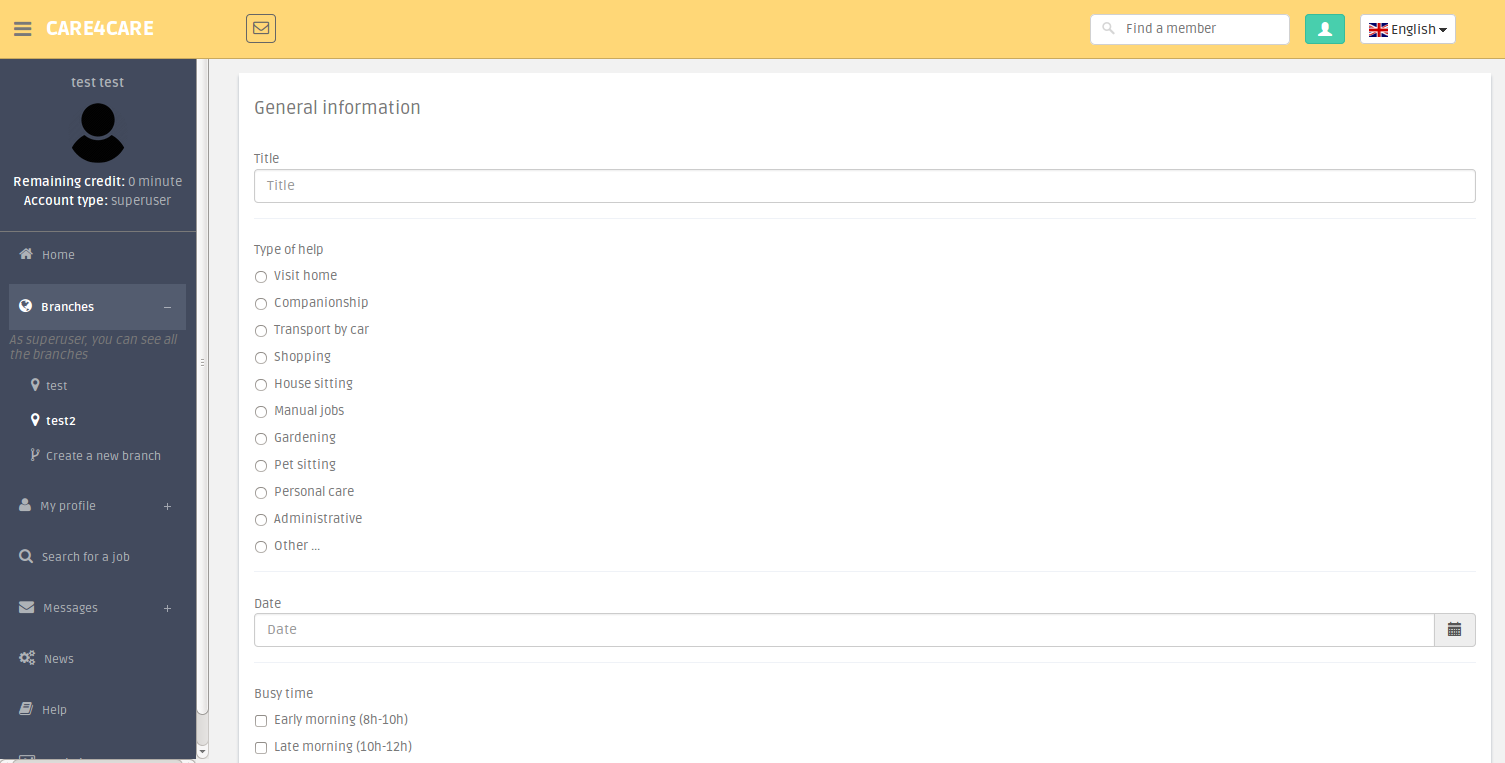
\includegraphics[width=\textwidth]{img/dem4.png}
   \caption{Ask: Step 4 - Fill in this form}
\end{figure}
\begin{figure}[!ht]
   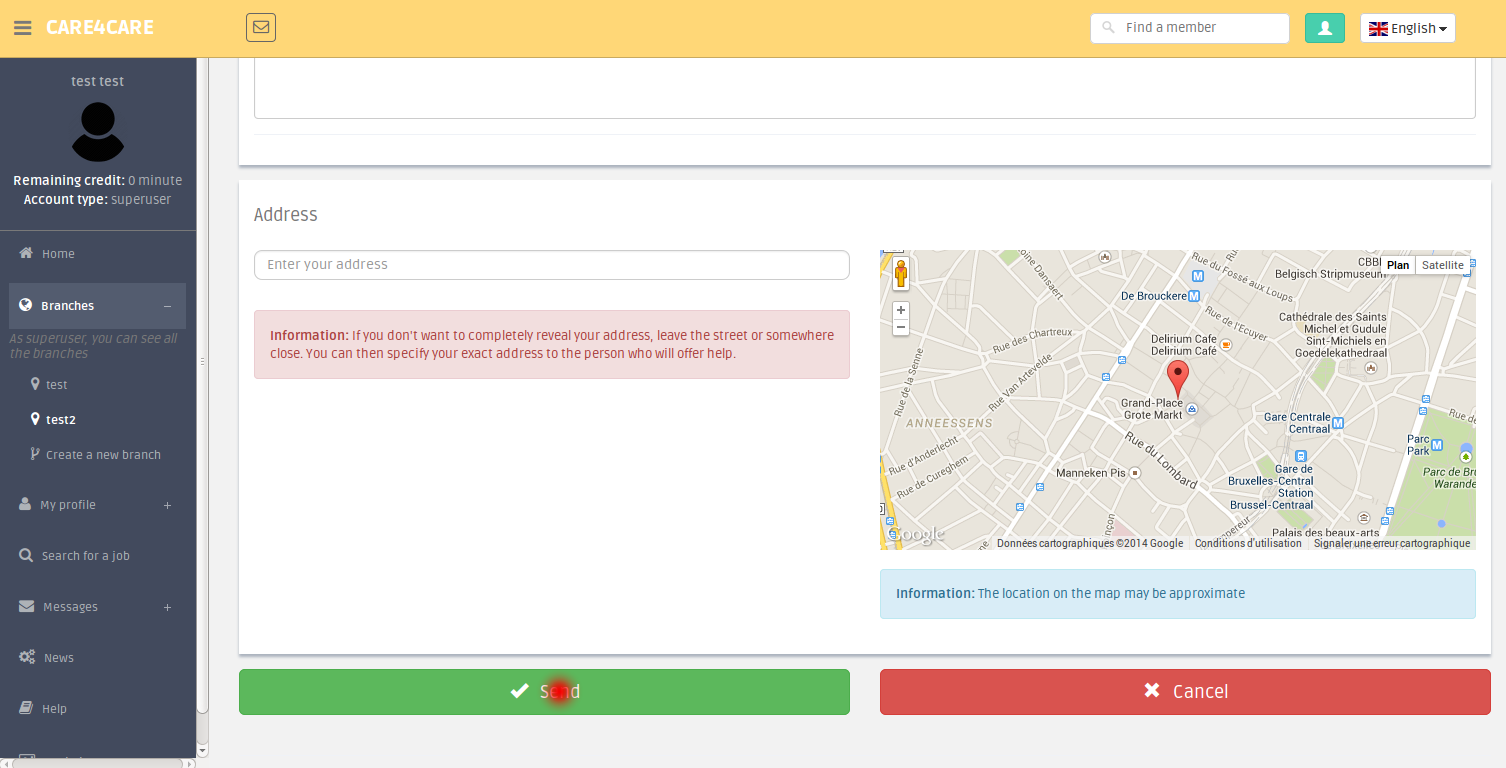
\includegraphics[width=\textwidth]{img/dem5.png}
   \caption{Ask: Step 5 - Send demand}
\end{figure}

\clearpage
\subsection{Offer my help}
Follow the same steps for \textbf{Ask for help} but click on \textbf{Offer my help} instead of I need help.


\subsection{Favorites and My network}
\subsubsection{What are the differences?}
You can make demands addressed only to people in \textbf{Favorites}.
People in \textbf{My network} will see more informations about you.
\subsubsection{How to add people in Favorites?}
Go to: \textbf{My profile}.
\begin{figure}[!ht]
   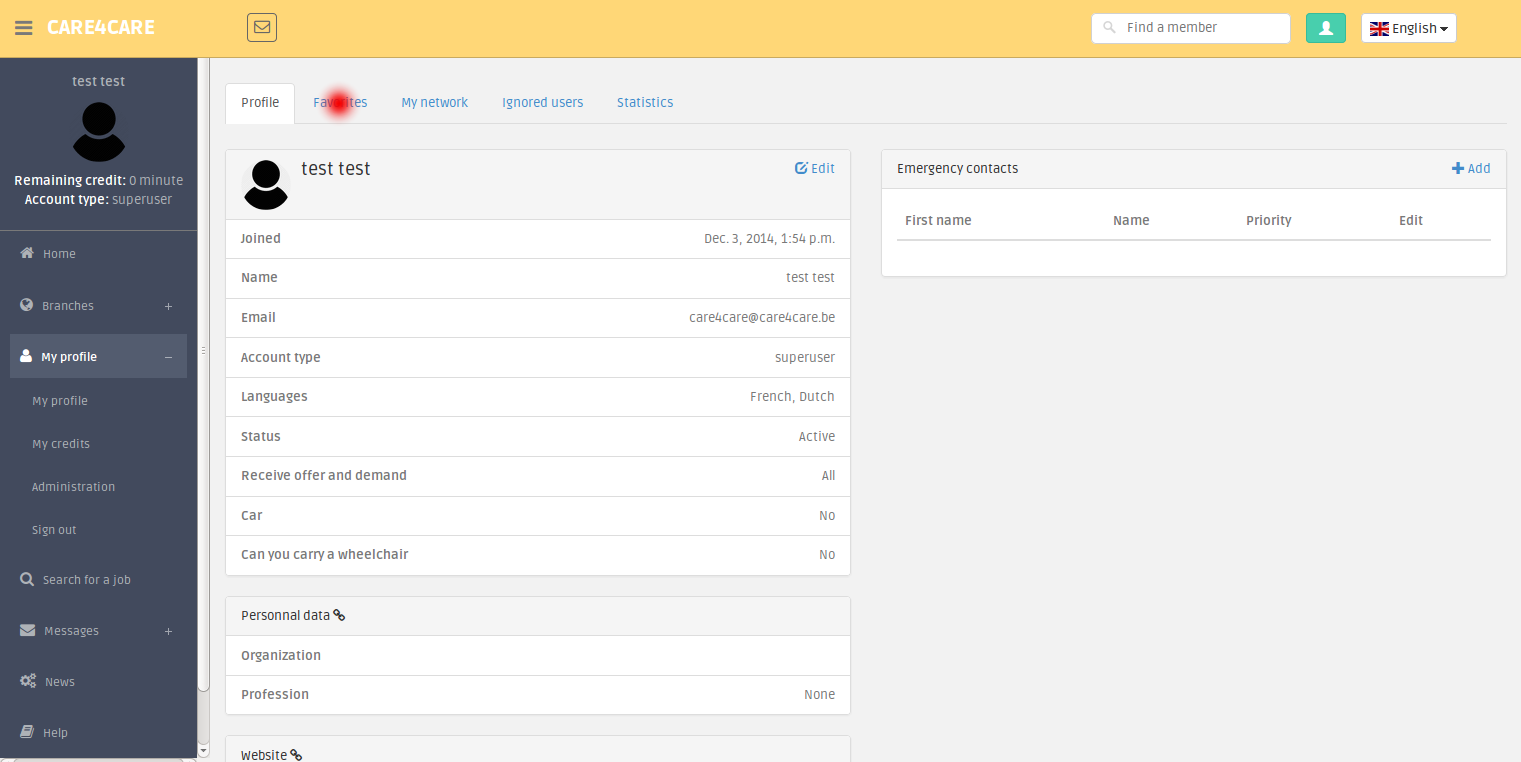
\includegraphics[width=\textwidth]{img/fav1.png}
   \caption{Favorites: Step 1}
\end{figure}
\begin{figure}[!ht]
   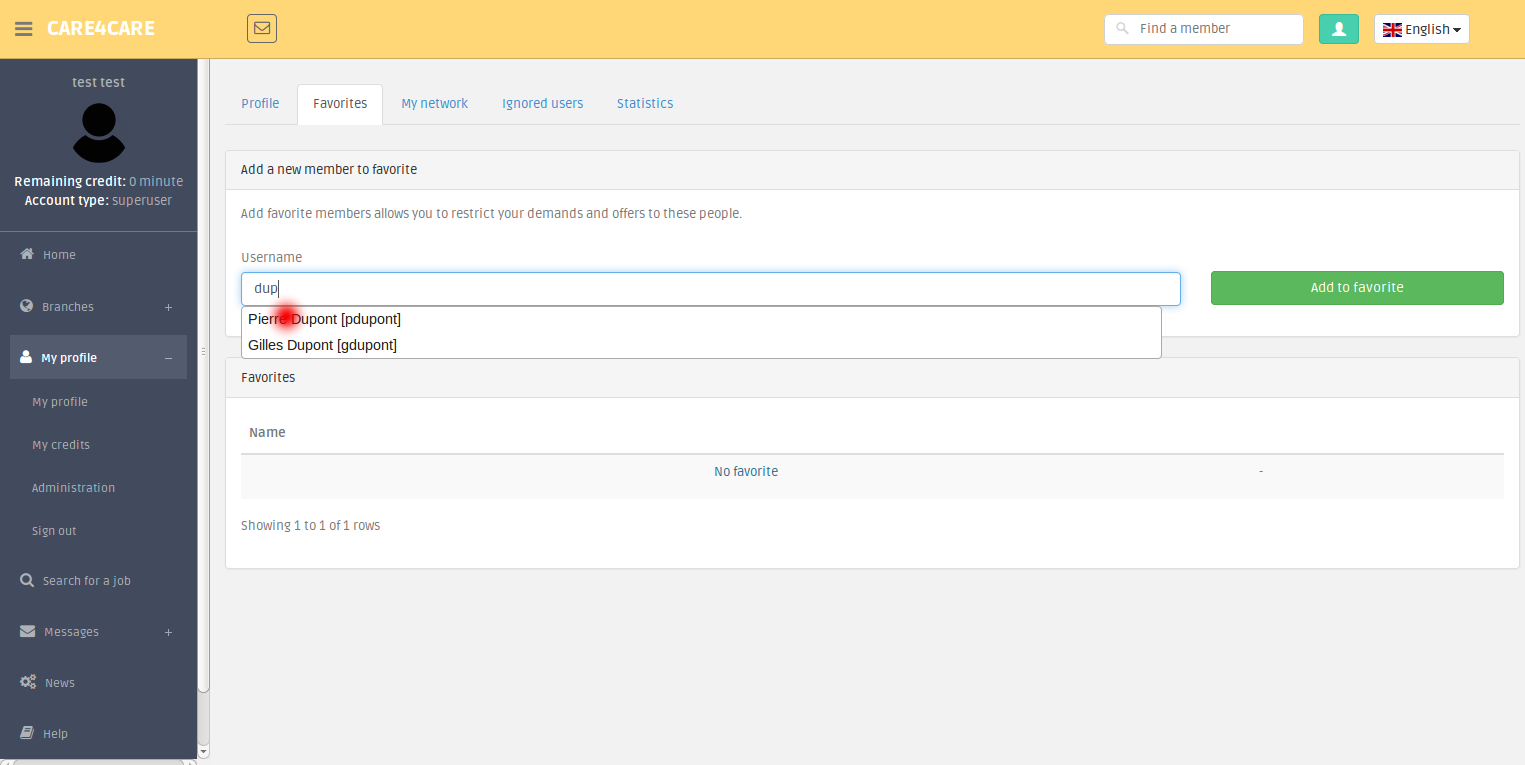
\includegraphics[width=\textwidth]{img/fav2.png}
   \caption{Favorites: Step 2 - Fill the field and select the user}
\end{figure}
\begin{figure}[!ht]
   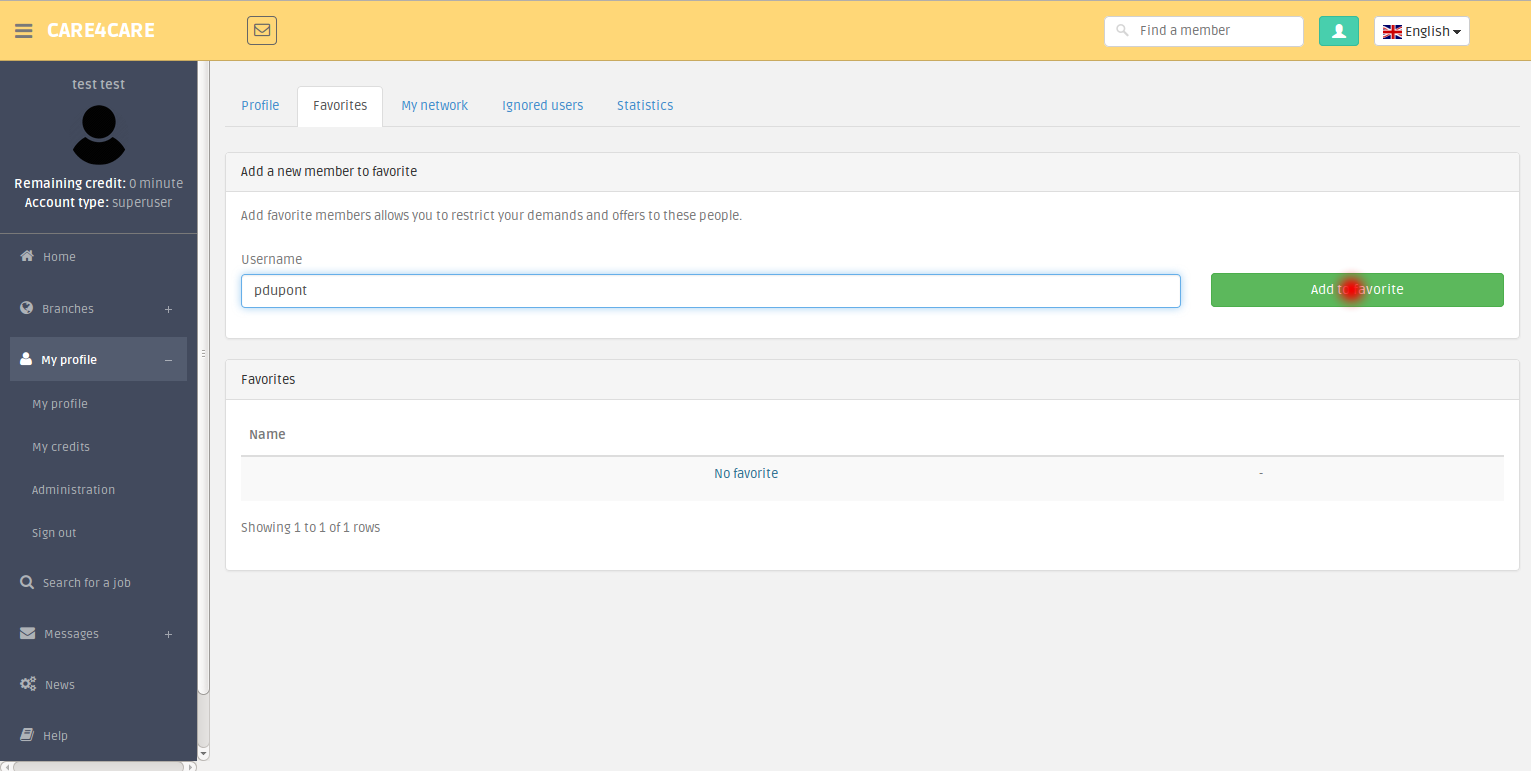
\includegraphics[width=\textwidth]{img/fav3.png}
   \caption{Favorites: Step 3}
\end{figure}
\begin{figure}[!ht]
   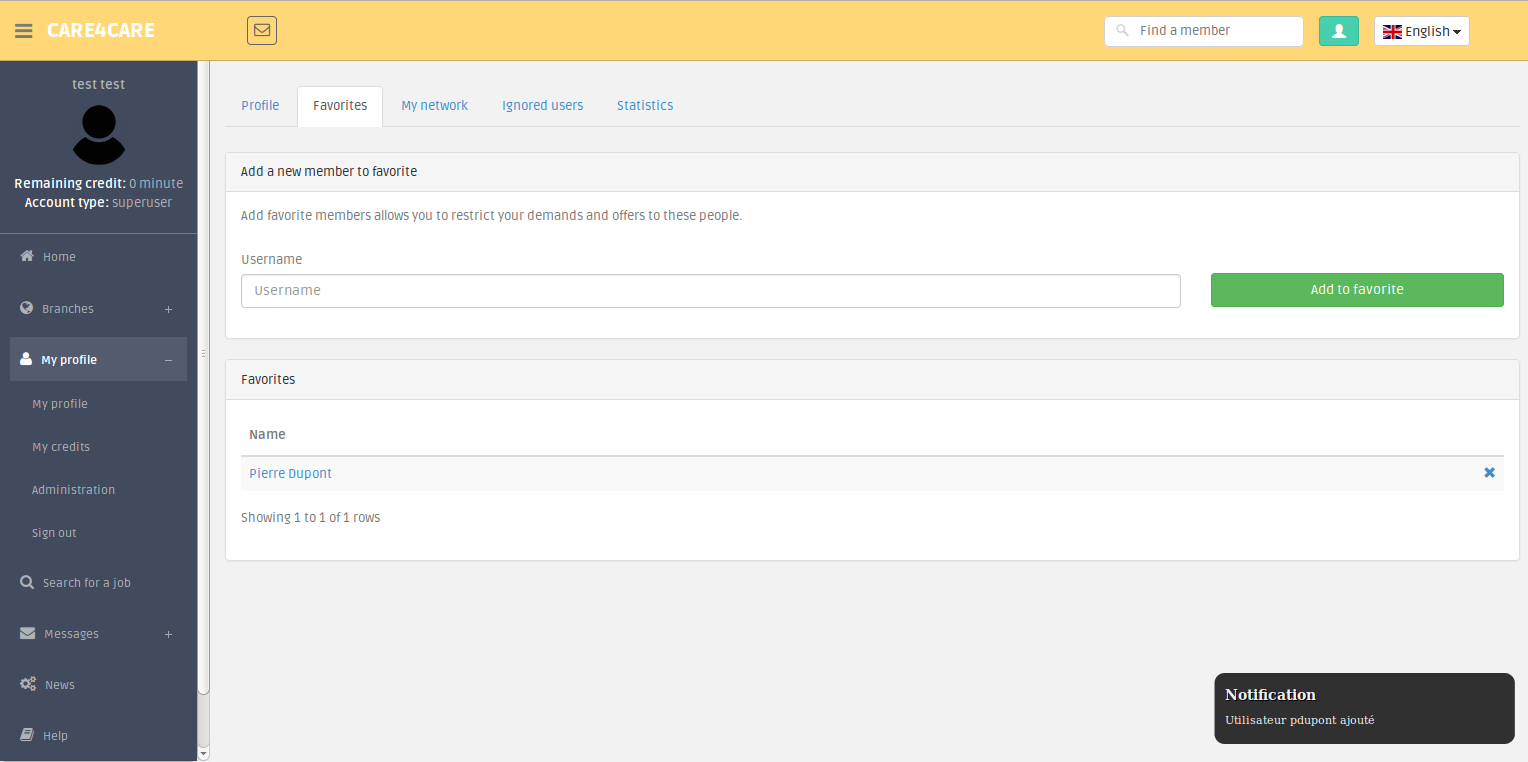
\includegraphics[width=\textwidth]{img/fav4.png}
   \caption{Favorites: Result}
\end{figure}
\subsubsection{How to add poeple in My network}
Follow the same steps as favorites but first click \textbf{My network} instead of \textbf{Favorites}.

\clearpage
\subsection{Messages}
Click on the small mailbox beside \textbf{Care4Care} or click on \textbf{Messages} in the menu, then choose, for example, \textbf{Inbox}, will lead you to the same page. 
\subsubsection{Read a received message}
\begin{figure}[!ht]
   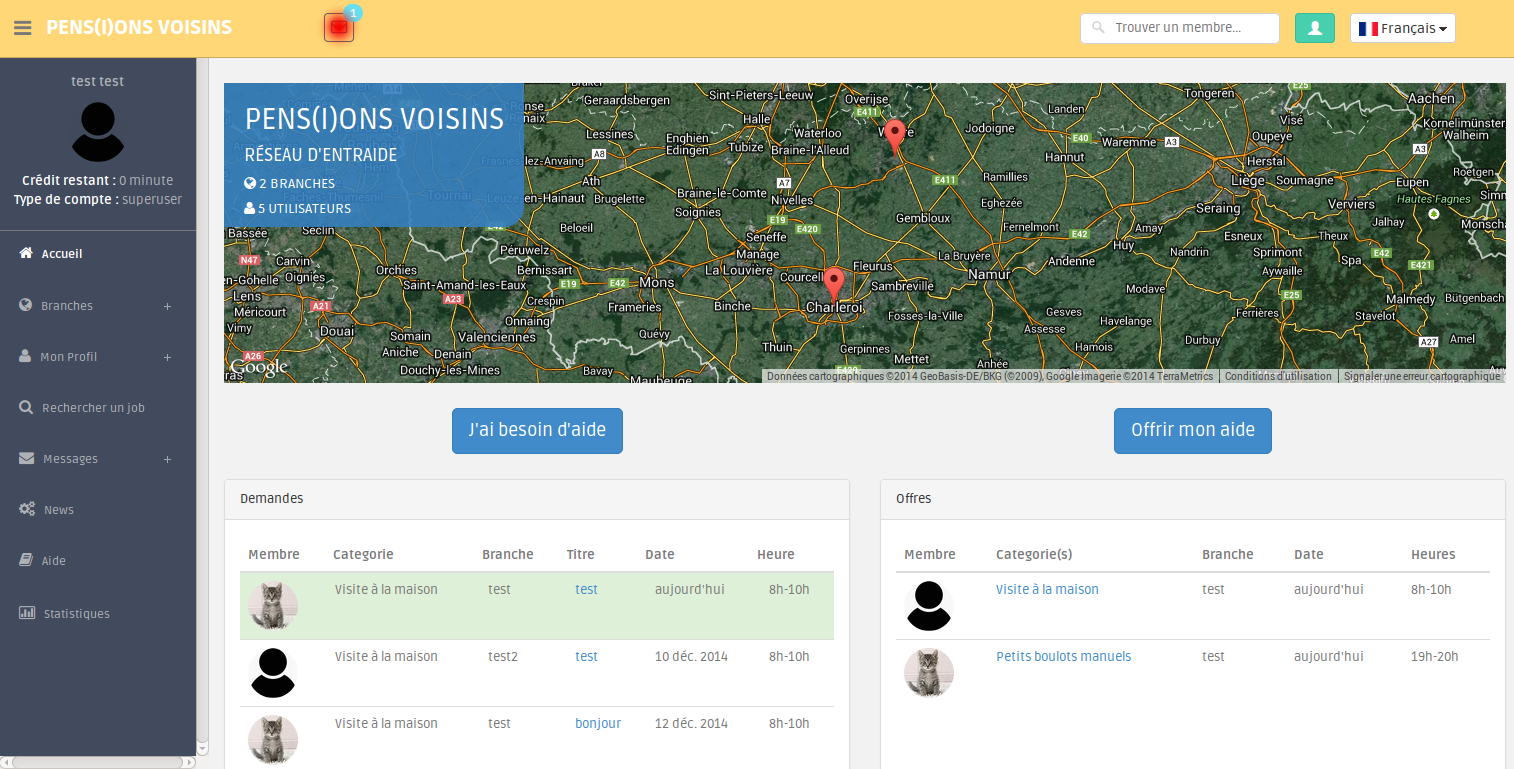
\includegraphics[width=\textwidth]{img/mess1.png}
   \caption{Message: Step 1}
\end{figure}
\begin{figure}[!ht]
   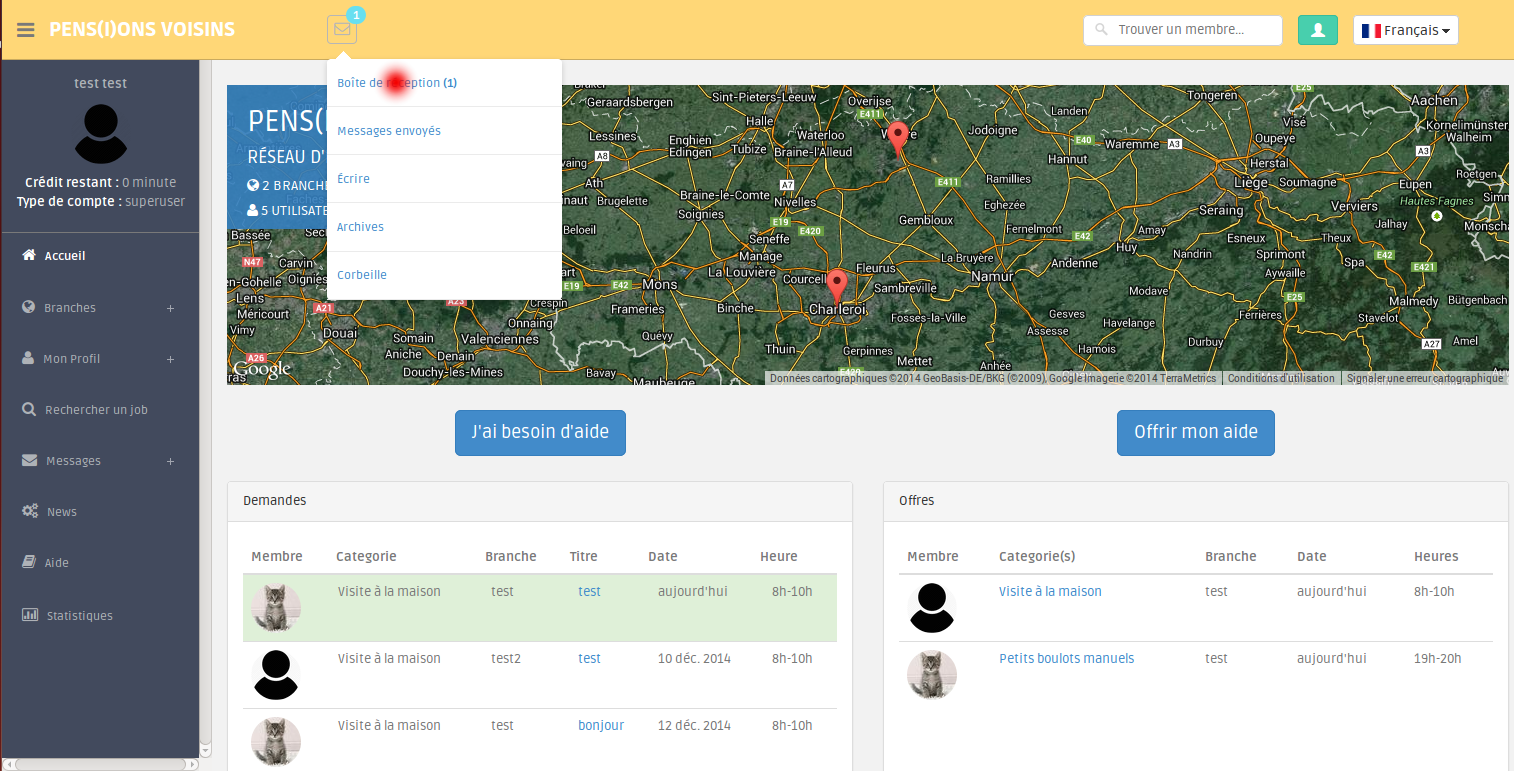
\includegraphics[width=\textwidth]{img/mess2.png}
   \caption{Message: Step 2}
\end{figure}
\begin{figure}[!ht]
   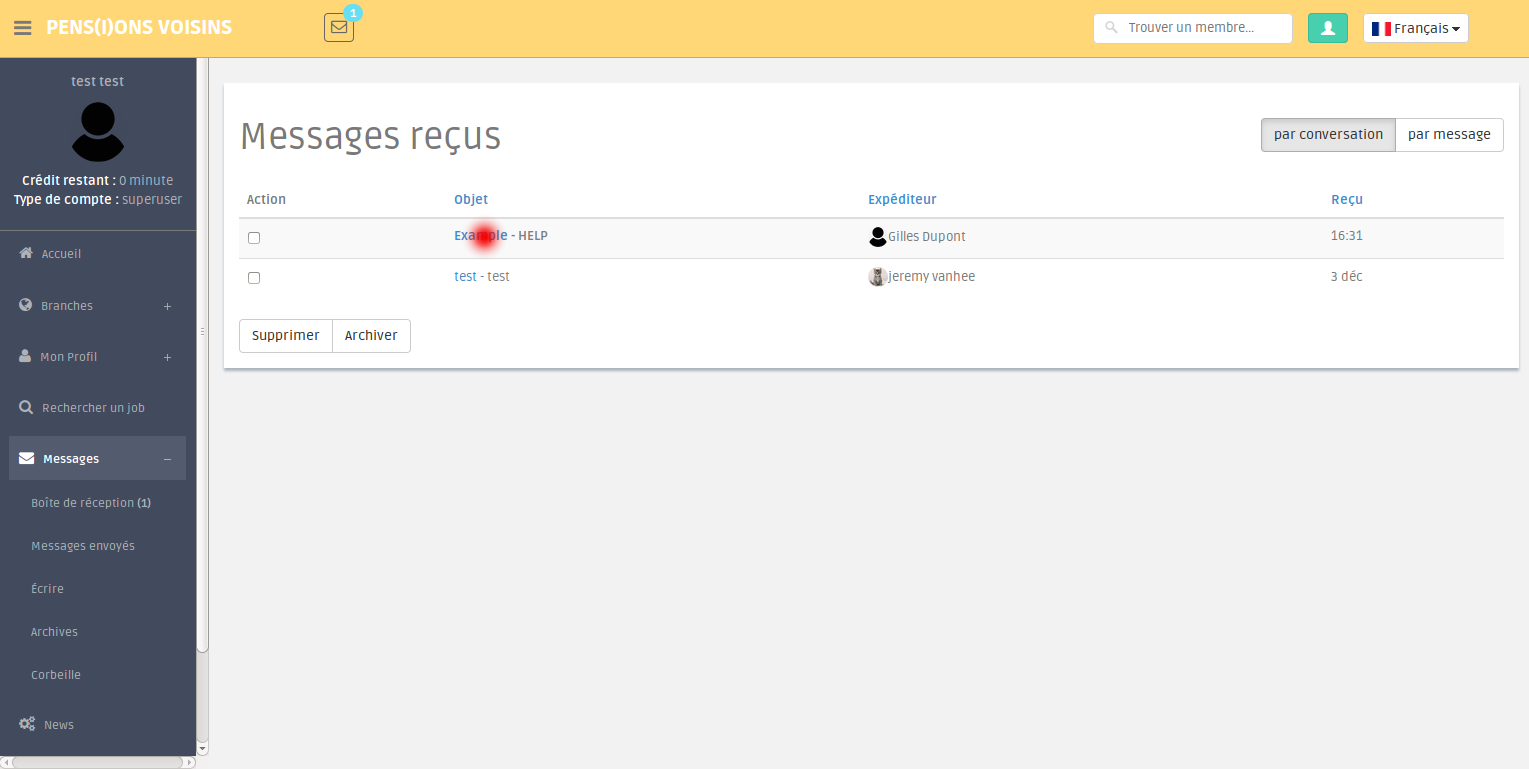
\includegraphics[width=\textwidth]{img/mess3.png}
   \caption{Message: Step 3}
\end{figure}
\begin{figure}[!ht]
   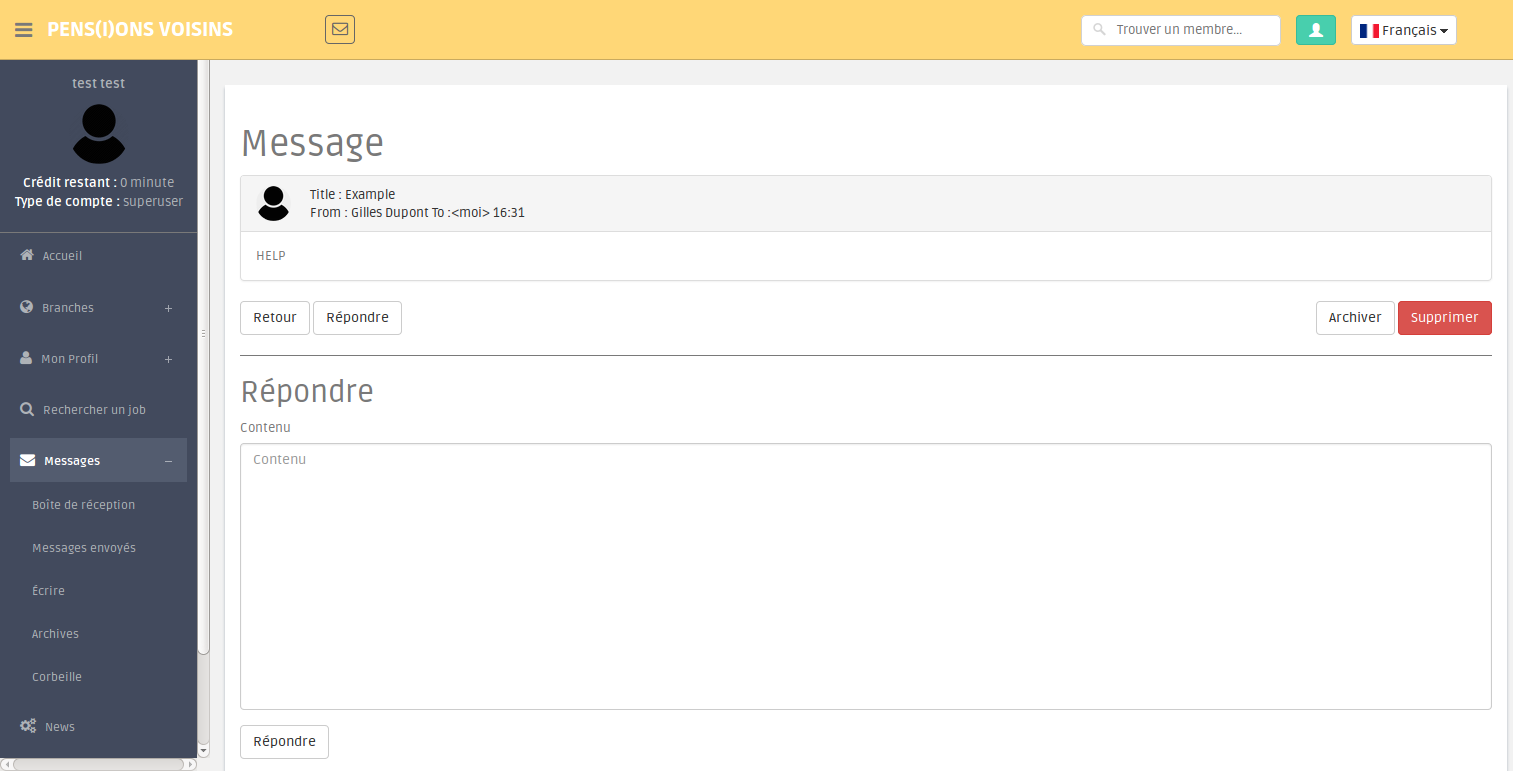
\includegraphics[width=\textwidth]{img/mess4.png}
   \caption{Message: Result}
\end{figure}
\section{What's inside the database}
This describe what is inside the database installed on the website: http://care4demo.tycale.be.
\subsection{Members and relations}
The passwords of all those users is ``care4care"
\begin{itemize}
	\item ``care4care" is the admin of the website;
	\item ``MHeraly" is a member, banned of the branch ``Bruxelles";
	\item ``VVelghe" is the branch officer of the branch ``Bruxelles". He has asked help for walk his dog;
	\item ``BLacasse" is a member of the branch ``Bruxelles". He offers his help and helps ``TGerondal";
	\item ``TGerondal" is a verified member, and he is in the branch ``Bruxelles". He is helped by ``BLacasse";
	\item ``DGenon" is a member of the branch ``Bruxelles", and he is volunteer to help ``VVelghe";
	\item ``AMoyaux" is a member of the branch ``Bruxelles", he is asking for help and has ``APaulus" and ``VVelghe" in his network;
	\item ``JVanhee" is a member of the branch "Bruxelles". He is asking for help for shopping and repairing his dishwasher.  ``VVelghe" and ``AMoyaux" are his favorites;
	\item ``APaulus" is a non-member. He can see the informations of ``JVanhee" and ``AMoyaux" because he is in his personal network. He can see the informations of ``MHeraly" because he is in the personal network of ``AMoyaux".
\end{itemize}

\end{document}